\documentclass[reprint,aps,prb]{revtex4-1}

% Language and font encodings
\usepackage[english]{babel}

% Useful packages
\usepackage{graphicx}
\usepackage{subfig}
\usepackage{amsmath,amsfonts,amssymb,amsthm}
\usepackage{mathtools,braket}
\usepackage{tikz}
\usepackage{xifthen}
%\pgfplotsset{compat=1.15}

%\usepackage[markup=underline]{changes}
%\usepackage[final]{changes}
%\definechangesauthor{dal}
%\definechangesauthor{gen}

% notation for standard math
\renewcommand{\d}{\partial}
\newcommand{\half}{\frac{1}{2}}
\newcommand{\dd}{{\rm d}}
\renewcommand{\r}{{\bf r}}
\newcommand{\br}{\bar{\bf r}}
\renewcommand{\AA}{{Angstr\"om}}
\newcommand{\x}{{\bf x}}
\newcommand{\eps}{\epsilon}
\newcommand{\bomega}{\bar\omega}
\newcommand{\bbomega}{\bar{\bomega}}
\newcommand{\ii}{\mathrm{i}}
\newcommand{\intdef}[3]{\int_{#1}^{#2} \dd {#3}}
\newcommand{\intover}[1]{\int_{-\infty}^{+\infty} \dd {#1}}
\newcommand{\sint}{\mathrlap{\displaystyle\int}
\mathrlap{\textstyle\sum}
\phantom{\mathrlap{\displaystyle
\int}\textstyle\sum}}

% notatiotion for equation environments
\newcommand{\be}{\begin{equation}}
\newcommand{\ee}{\end{equation}}
\newcommand{\ba}{\begin{eqnarray}}
\newcommand{\ea}{\end{eqnarray}}
\newcommand{\baa}{\begin{align}}
\newcommand{\eaa}{\end{align}}
\newcommand{\nn}{\notag}
\newcommand{\qq}{\qquad}
\newcommand{\lb}{\label}
\newcommand{\mat}[1]{\begin{pmatrix} #1\end{pmatrix}}

% notation for the operators
\newcommand{\op}[1]{\hat {#1}}
\newcommand{\sop}[1]{\op{\op {#1}}}
\newcommand{\commutator}[2]{\left[ {#1} , {#2} \right]}
\newcommand{\trace}[1]{\mathrm{tr}\left(#1\right)}
\newcommand{\argument}[1]{\ifthenelse{\isempty{#1}{}}{}{(#1)}}
\newcommand{\matop}[1]{\mathbf{#1}}
\newcommand{\optr}[1]{\check #1}
\newcommand{\opskew}[1]{{\op {#1}}_{\perp}}

% notation for the states
\newcommand{\tket}[1]{| \tilde #1 \rangle}
\newcommand{\tbra}[1]{\langle \tilde #1 |}
\newcommand{\brket}[2]{\langle  #1 | #2 \rangle} %standard braket
\newcommand{\tbraket}[2]{\langle \tilde #1 | #2 \rangle}
\newcommand{\ketbra}[2]{| #1 \rangle \langle #2 |}
\newcommand{\tketbra}[2]{| #1 \rangle \langle \tilde #2 |}
\newcommand{\sket}[2]{| #2)^{#1}}
\newcommand{\sbra}[2]{( #2|_{#1}}
\newcommand{\sketor}[2]{| #2]^{#1}}
\newcommand{\sbraor}[2]{[ #2|_{#1}}
\newcommand{\sbraket}[2]{\braket{\op{#1} | \op{#2}}}
\newcommand{\dket}[1]{\Bigl| #1 \Bigr)}
\newcommand{\dbra}[1]{\Bigl(#1 \Bigr|}
\newcommand{\dbraket}[2]{\Bigl(#1 \Bigl| #2 \Bigr)}
\newcommand{\dketor}[1]{\Bigl| #1 \Bigr]}
\newcommand{\dbraor}[1]{\Bigl[#1 \Bigr|}
\newcommand{\hket}[1]{| #1 ]}
\newcommand{\hbra}[1]{[ #1 |}
\newcommand{\hbraket}[2]{[#1 | #2 ]}

% special operators
\newcommand{\dmnot}{\op{\rho}_0}
\newcommand{\dm}{\op{\rho}}
\newcommand{\hnot}{\op{H}_0}
\newcommand{\hone}[1]{\op{H}_1\argument{#1}}
\newcommand{\transition}[1]{\op T_{#1}}
\newcommand{\excite}[2]{\op e_{{#1}{#2}}}
\newcommand{\decay}[2]{\op d_{{#1}{#2}}}
\newcommand{\Liouv}{\sop{\mathcal L}}
\newcommand{\Liouvnot}{\sop{\mathcal L_0}}
\newcommand{\coupl}{\sop{\mathcal K}}
\newcommand{\honetmp}[1]{\op{H_1}\argument{#1}}
\newcommand{\identity}{\op{\mathbb I}}
\newcommand{\rmat}[1]{\optr R}
\newcommand{\fscd}[1]{\mathrm{Im}\ket{f_p^{\mathbf r_j}(\omega)^{#1}}}
\newcommand{\GH}{\op G_{\op T}}

\captionsetup{justification=centerlast}

\begin{document}

%\preprint{APS/123-QED}

\title{Locality and Computational Reliability of Linear Response Calculations for Molecular Systems}
\author{Marco D'Alessandro}
\affiliation{Istituto di Struttura della Materia-CNR (ISM-CNR), Via del Fosso del Cavaliere 100, 00133 Roma, Italia}
\author{Luigi Genovese}
\affiliation{Laboratoire de Simulation Atomistique (LSim), INAC, CEA-UGA, 17 Av. des Martyrs,
38054 Grenoble, France}
\date{\today}

\begin{abstract}
By performing a critical analysis of the fundamental equations of linear-response (LR) formalism in molecules,
we explore the interplay between locality of the response density operator and  numerical convergence of LR-related quantities.
We show that for frequencies below the first ionization potential (IP) of the system, it is possible to express the response density by employing localized states only.
Above this threshold energy, such a locality property cannot be achieved.
Such considerations may be transposed in terms of the molecule's excited states. We show that not all the system's excitations can be considered on equal footing.
There is a discrete sector of excitations -- which may extend above IP -- that can be parametrized by observable, localized states, which can be computationally expressed with high precision, provided an adequate level of completeness.
We present indicators that can help to quantify such potential observable property of an excitation, that can be evaluated
in any discretization scheme.
The remaining excitation modes belong to a continuum spectrum that, on the contrary, is not directly associated to observable properties and can only be effectively represented in a given computational setup.
Such considerations are important not only for reproducibility of the results among different computer codes
employing diverse formalisms, but also in view of providing a deeper understanding on the impact of models'
approximations on the scientific outcomes of the simulation.
\end{abstract}

%\pacs{Valid PACS appear here}
\maketitle

\section{Introduction}

For a theoretical approach that is based on numerical calculations, for which no analytic reference solution exists,
reducing the computational uncertainty is the only possible way to shed light on the predictivity power of the
model. In other terms, the ``accuracy'' of a result with respect to experimental data may be reliably quantified
only when the computational uncertainty is guaranteed to be significantly lower than the found discrepancy.
For communities employing Density Functional Theory (DFT), the need of such a ``calibration'' of computer codes has led to the DeltaCodes project~\cite{deltaTest2016}.
This project represents a remarkable example of precision-driven initiative where a grassroot community of code-owners struggled to extract
well-defined computational results in the context of DFT calculations. Ground-State quantum mechanical quantities
as lattice constants and bulk modulus of elementary crystals extracted from different codes were compared with each other, with the objective of reducing the uncertainties on such data, and in some sense, to define a \emph{calibration} procedure for a Solid-State Physics DFT code.
Any other code able to extract the same quantities with the same approximations may be compared with the
results of the community in order to assess its computational reliability.

The problem is even more stringent for calculations that refer to quantities \emph{beyond} ground state, like
for instance the time-dependent density functional theory (TDDFT) \cite{casida1995,runge1984,onida2002},
from which quantities like optical excitations or polarizability tensors
of a given system may be studied and put in relation with experimental data.
Here also, a plethora of computational approaches exist, that employ different numerical formalism and
basis sets, and it will be of great importance to identify quantities that can be ``measured'' in a given model, to assess
and quantify their computational uncertainty.

In this paper, we focus our attention to Linear-Response treatments of \emph{molecular} systems,
in particular referring to LR-TDDFT calculation. We will investigate the impact that \emph{open} (i.e. Isolated) Boundary Conditions (BC), that are imposed to the system, will have on the computational evaluation of LR quantities.
We perform analytic considerations on the equations beyond LR treatment and discuss the interplay between reproducible LR quantities and the \emph{locality} of the related objects. Such considerations will enable us to distinguish quantities that \textit{a priori} can be compared among different treatments - and therefore tested for reproducibility - from others that would \emph{explicitly} depend of the employed computational treatment.

It is indeed relatively easy to have converged indicators for numerical Ground State (GS) quantities: on one side, the variational theorem
guarantees that the lower the GS energy, the more precise the numerical result; on the other side, GS quantities of molecular system  can be expressed
only in terms of localized (i.e. bound) states. These considerations make relatively easy to increase the basis set completeness in view of the extraction of reference results.

We will see in what follows that the situation is not as simple in the context of LR. Indeed we will show that the response density -- even for molecular systems -- looses its localized behaviour for high frequencies, independently on the nature of the specific system and perturbation. Furthermore, we will demonstrate that to increase the basis set completeness, delocalized oscillatory degrees of freedom cannot be excluded \textit{a priori}, even in the localized regime.

We will also see that the reliabilty of the convergence criteria that can be established for LR -- where no variational theorem exists -- depends explicitly on the target frequency range and on the features of the numerical basis set.

% This analysis evidences that the description of molecular systems beyond the ground state unavoidably leads to the inclusion of delocalized
% degrees of freedom above a specific energetic threshold. Moreover on the basis of this analysis we can assess something about the reliability of the results provided by computational setups able to explicit include the presence of delocalized degrees of freedom compared
% to the ones in which these degrees of freedom are excluded by design.

The paper is organized as follows.
Initially we will inspect how the question of reproducibility may be expressed
for ground state calculations of molecules.
Following these guidelines, we will then move to LR equations,
by first considering the equations of motion of the response density operator, given
the application of a perturbing field.
Then we will consider the behavior of the ``free oscillations'', i.e. the excited states
of the molecule.
Our considerations will also reveal useful for the understanding of the \emph{analytic structure} of LR quantities like
the linear susceptibility of the system (i.e. the reducible polarizability).
We support our considerations with numerical results on simple LR-TDDFT quantities.
For readability purposes, the details of each calculation are explained in Appendix~\ref{compdetails}.

Although we refer, as anticipated, to TDDFT models, such considerations might also be transposed to Many-Body Perturbation Theory
approaches, in the context of Quasi-Particle equations.

\subsection{Long range behavior of the eigenvalue solution of the Schr\"odinger equation}
\label{SEopenSystem}

Let us start our discussion by reviewing some well-known concepts of quantum mechanic under a perspective that will turn out to be very useful 
in the forthcoming considerations about linear-response quantities. In particular we revisit the impact that the Isolated BC have on the solutions 
of the Schr\"odinger Equation.

Consider a (one-body) wavefunction $\ket{\psi}$ solution of the equation
$\op H\ket{\psi}=\eps\ket{\psi}$, where we split the Hamiltonian operator into the sum of
a kinetic $\op T$ and a potential $\op V \equiv \op H - \op T$ term.
In view of discussing the impact of the BC, it is instructive to transform
the Schr\"odinger equation in a scattering problem, by writing
\be\lb{SEHelmholtz1}
\ket{\psi} = \GH(\eps)\ket{\op V\psi}\;,
\ee
where we have introduced the Green function of the Helmholtz operator $\GH(\eps) = (\eps-\op T)^{-1}$,
resolvent of the free-particle Hamiltonian $H_s \equiv \op T$.

When describing the Ground State of a molecule, we suppose that the potential operator, even if non-local,
can be effectively restricted on wavefunctions that can be considered as nonzero only on a
bounded domain. In other terms, a molecule can be associated to a ``scatterer'' that has a \emph{finite}
spatial extension; if a state $\ket{\psi}$ is localized, it will be the same for the ket $\ket{\op V \psi}$, though
perhaps in a larger region.
For a computational analysis of the problem, this property is fundamental in the choice of the numerical treatment as we know that
computational basis sets
that are tailored to express asymptotically vanishing wavefunctions are better suited for the solution of the problem.

This fact is made apparent by the expression of
the kernel of $\GH(\eps)$ in the coordinate representation.
When dealing with Isolated BC, it is easy to see that the solution of Eq.~\eqref{SEHelmholtz1}
can be expressed by:
\be\lb{HelmholtzKernelDef1}
\bra{\r} \GH(\eps) \ket{\r'} = \frac{1}{4\pi} \begin{cases}
\frac{e^{-\alpha|\r - \r' |}}{|\r- \r' |} \;,\; & {\textrm for}\; \eps  < 0\; \\
\frac{e^{\ii \alpha |\r-\r' |}}{|\r-\r' |} \;, & {\textrm for} \; \eps \geq 0
\end{cases} \;,
\ee
where $\alpha = \sqrt{2|\eps|}$.

From the above expressions we can see that, for molecular systems,the value $\epsilon=0$
represents a \emph{threshold}~\footnote{The threshold value in general should correspond to asymptotic value of the potential at infinity.}
energy that separates two different classes of solutions.
Negative-energy solutions are \emph{localized}, i.e. they exhibit bound-state behavior far away from the scatterer.
These are bound states and, by means of their normalizability, they are associated to \emph{discrete}, well-defined energies.
The bound states can be of course labelled by quantum numbers that are defined by the properties of the scatterer, namely the
symmetries of the potential $\op V$.
In a computational discretization of the Schr\"odinger equation, such states can be in principle expressed with arbitrary precision,
provided that the numerical treatment offers the adequate level of completeness.
Being discrete and well-identified, the bound-state energies are a property of the molecule and can be associated to \emph{observable}
quantities. The values of their energies can be compared among different treatments and it is in principle possible to
provide reference results on them.

On the other hand, positive energy solutions behave differently. Even though the potential is localized the associated Helmholtz kernel is a spherical wave and its convolution with the source term provides a delocalized wavefunction $\psi(\r)$ in the whole space.
As they cannot be normalized they belong to the essential spectrum of the Hamiltonian operator and form a \emph{continuum} of states.
Outside of the support of the $\ket{\op V \psi}$ the solutions of Eq.~\eqref{SEHelmholtz1} can be put in bijection with the eigenstates of the
free-particle Hamiltonian $\op H_s$. For positive energies, the quantum numbers of the eigenstates are determined by the Laplacian operator,
regardless of the particular features of the potential.

It is easy to see from these concepts that a computational treatment that is tailored for the discretization of bound states
will not be as effective for continuum states, due to the different long-range asymptotic behavior - which in turn is a clear consequence of the
BC of the problem. In a numerical treatment, where we discretize the problem with a \emph{finite}
number of degrees of freedom, we will only have access to a \emph{pseudo}-continuum of states,
whose energy values and density of states will depend on the representation of the kinetic operator
in the basis set. As a consequence, the set of eigenstates with $\epsilon > 0$ expressed in a given computational setup depends on the features of the employed basis set.

A direct numerical evidence of this problem has been discussed in \cite{boffi2016}, where the authors analyze the effects of a finite basis set on the
occupied and virtual orbitals of a molecular system and establish a clear correspondence between the orbital localization character,
and the independence of its energy with respect to the basis set.
Furthermore, it is clearly shown that the energies of the unbound orbitals are not stable with respect to parameters like the size of the computational domain.

\section{Fluctuation states. A localization argument for the response density}
\label{FluctuationState}
It is evident that the arguments presented above have a limited interest for the study
of Ground State quantities of molecules. By definition, all these quantities can be expressed as a
functional which \emph{entirely} depends on bound states. As an illustration it is sufficient to recall
the Hohenberg-Kohn theorem that states that the Ground-State (GS) energy is a functional of the GS
charge density $\dmnot$. For molecular systems that are electronically stable (i.e. no anionic or metastable configurations),
such quantity is localized, in the sense of the above section. Stated otherwise,
\emph{there is no need to express efficiently any portion of the continuum spectrum} to have a reliable GS treatment of molecules.

Let us now inspect the case of LR calculations.
In this framework one consider the unperturbed Hamiltonian $\hnot$ and assume that
the GS density $\dmnot$ is accessible and expressed in a given computational treatment.
The linear response formalism allows us to evaluate the modification of the expectation value of a generic observable induced by a
time (or frequency)-dependent perturbing field $\op\Phi(\omega)$ acting on the system.
This quantity, written in the frequency domain, can be expressed through the evaluation of the \emph{linear response functional}
\be\lb{LinearResponseFunctDef1}
\braket{\delta\op O}_\Phi(\omega) = \trace{\dm'_\Phi(\omega)\op O} \;,
\ee
where $\op O$ represents the observable\footnote{For a sake of concreteness, we are limiting our considerations to observables that do not explicitly depend on time} under inspection
and we have introduced the \emph{response density operator} $\dm'_\Phi(\omega)$ that codifies the modification of $\dmnot$ induced by the perturbation $\op\Phi(\omega)$.

The response density operator is expressed as the first-order variation of $\dmnot=\sum_{\{p\}} \ket{\psi_p} \bra{\psi_p}$, where the set $\{\ket{\psi_p}\}$ denote the
occupied states, \emph{i.e} the subset of the bound eigenstates\footnote{In what follows we will assume that the set of states $\{\ket{\psi_p}\}$ are described by real
functions, when projected in the $\r$-representation.} of $\hnot$ with (negative) energy $\eps_p$ lower than the Fermi level. Using this notation we denote the energy of the HOMO level
as $\eps_h$ and identify the value of the first ionization potential with IP~$\equiv|\eps_h|$.

The response density satisfies an equation of motion written in the form of a quantum Liouville operator (for example see \cite{baroni2008})
\be\lb{LiouvillianRhopomegaDef1}
\left(\omega - \Liouv\right) \dm'_\Phi(\omega) =  \commutator{\op\Phi(\omega)}{\dmnot} \;.
\ee
The Liouvillian superoperator $\Liouv$ for self-consistent systems is expressed as the sum of the unperturbed part $\Liouvnot$ plus a coupling term $ \coupl$. The action of these
terms reads, respectively
\be\lb{LiouZeroDef1}
\Liouv \op O \equiv \left(\Liouvnot + \coupl \right) \op O = \commutator{\hnot}{\op O} +\commutator{\op V'[\op O]}{\dmnot}  \;,
\ee
where $\op V'[\op O] \equiv \int \dd \r \dd \r'\frac{\delta \op V[\dmnot]}{\delta \rho(\r,\r')} O(\r,\r')$ encodes the response of the $\dm$-dependent potential to a modification of the density operator.
The inspection of the linear order time evolution of the eigenstates of $\hnot$ evidences that the response density acts as a transition
operator, linking the occupied and empty subspaces of $\hnot$.
An operator $\op O_\perp$ with this feature satisfy the \emph{transverse} condition
\be\lb{RhopTransverseDef1}
\op O_\perp \equiv
\dmnot\op O \op Q_0 + \op Q_0 \op O\dmnot \;,
\ee
where $\op Q_0=\identity-\dmnot$ is the projector in empty subspace of $\hnot$
(for more details see Appendix~\ref{LiouvillianAction}).
In other terms, the condition $\dm'_\Phi = \dm'_{\Phi\,\perp}$ holds.

We can therefore introduce an explicit representation of the
response density parametrized as
\be\lb{rhoPrimeFluctuationStateDef1}
\dm'_\Phi(\omega) = \sum_p\left(\ketbra{\psi_p}{f_p^\Phi(-\omega)} + \ketbra{f_p^\Phi(\omega)}{\psi_p}\right) \;.
\ee
Here we have introduced the set of $\omega$-dependent \emph{fluctuation states} (FS)
$\ket{f_p^\Phi(\omega)} = \dm'_\Phi(\omega) \ket{\psi_p}$, that have values in the unoccupied subspace of $\hnot$.
However, non-hermiticity of $\dm'_\Phi(\omega)$ implies that the
fluctuation states are complex quantities.

An analysis of the Liouville equation \eqref{LiouvillianRhopomegaDef1} for the response density written in this fashion evidences that the equations of motion of fluctuation states  are
written as a modified Sternheimer equation~\cite{mahan1980,giustino2012,giustino2014}
\be\lb{fluctuationStateEqMotion1}
\left[\omega - (\hnot-\eps_p)\right]\ket{f_p^\Phi(\omega)} = \op Q_0(\op\Phi(\omega)+\op V'[\dm'_\Phi](\omega))\ket{\psi_p} \;,
\ee
and we observe that the first-order Hamiltonian contains,
apart from the perturbing field, a further term $\op V'[\dm'_\Phi]$ due to the density-dependence of $\hnot$.
It is easy to see that the solution of equation \eqref{fluctuationStateEqMotion1} can be recast in a scattering problem:
\be\lb{rhoPrimeFluctuationStateDef2}
\ket{f_p^\Phi(\omega)} = \GH(\omega+\epsilon_p)\left(\op V\ket{f_p^\Phi(\omega)} + \ket{s_p^\Phi(\omega)} \right)\;,
\ee
with the state
$
\ket{s_p^\Phi(\omega)} = \op Q_0(\op \Phi(\omega) +\op V'[\dm'_\Phi](\omega) )\ket{\psi_p}
$ as a source term.

Equation \eqref{rhoPrimeFluctuationStateDef2} is the convenient starting point to assess the localization properties of the FS as it is easy to see that, for each choice of $p$, the value $\omega = |\eps_p|$ represents the threshold level that governs the asymptotic behavior of the associated Helmholtz kernel.
As a ulterior \emph{stringent} hypothesis, let us now assume that the source term $\ket{s_p^\Phi(\omega)}$ is spatially localized, \textit{i.e.} its evaluation can be restricted on a bounded real-space domain.
Even when such locality argument holds true, for $\omega > |\eps_p|$,
the Helmholtz kernel behaves as a spherical wave and  gives raise to a $\ket{f^\Phi_p(\omega)}$ which is \emph{delocalized} in the entire real-space domain.
Such delocalization is an intrinsic consequence of the value of $\omega$, and does not depend on the particular choice of
$\op \Phi$.
Only for $\omega < |\eps_p|$ the kernel contains an exponential damping factor and $\ket{f^\Phi_p(\omega)}$ exhibits a bound-state behavior in the long range,
once again provided that the above locality arguments on $\ket{s_p^\Phi(\omega)}$ -- hence on $\op V'$ and $\Phi$ -- are valid.
These arguments demonstrate that for frequencies above the IP threshold energy, the response density operator cannot be expressed in terms of localized states. Locality of FS (and therefore of $\dm'_\Phi(\omega)$) can be only recovered for frequencies below such threshold.

\subsection{Localized behavior for static perturbations}
The locality property of the fluctuation state can be directly confirmed for static perturbations at $\omega=0$.
Let us consider a static perturbing operator $\op\Phi_s$ that can be restricted to a finite domain.
Any local operator, like \emph{e.g.} a static electric field $\mathbf F$, with associated scalar potential $\Phi_s[\mathbf F](\r) = -\mathbf F \cdot \r$, would satisfy such property.
We consider the perturbed Hamiltonian $\hnot[\dm_{\Phi_s}] + \op\Phi_s[\mathbf F]$, where $\dm_{\Phi_s}$ represents the GS density of the perturbed system, and assume that the
perturbation strength ($|\mathbf F|$ in the above example) is sufficiently small to be consistent with a LR treatment of the problem.
In this case, the occupied eigenfunction $\ket{\psi_p^{\Phi_s}}$ of the perturbed Hamiltonian can be extracted with traditional GS techniques,
as from the discussion around Eq.~\eqref{SEHelmholtz1}, they exhibit bound-state behavior.
\begin{figure}[t]
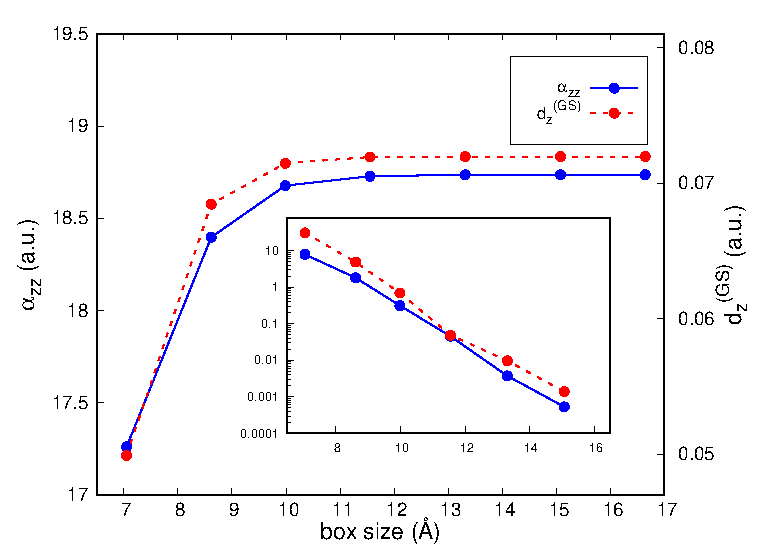
\includegraphics[scale=0.68]{Fig1_CO_statPolvsBox.eps}
\caption{\label{co_alphaStatic}(Color online) Convergence of the statical polarizability $\alpha_{zz}$ (blue continuous line) and of the ground state dipole $d_z$ (red dotted line)
of $CO$ molecule as a function of the size of the computational domain. The inset evidences the relative convergence (in percent) of the two quantities w.r.t. the corresponding value associated to the largest
box.}
\end{figure}

From the linearized Schr\"odinger Equation of the perturbed problem, it is easy to see that the FS at $\omega=0$ can be expressed
in terms of the corresponding bound state of the perturbed Hamiltonian, i.e.
$\ket{f_p^{\Phi_s}(0)} \simeq \op Q_0 \ket{\psi_p^{\Phi_s}}$.
For any value of $p$, the locality of the $\ket{f_p^{\Phi_s}(0)}$ therefore directly stems from the
bound-state behavior of $\ket{\psi_p^{\Phi_s}}$. As $\omega=0$ is by hypothesis
lower than any of the $|\eps_p|$, this is consistent with the above considerations.

Thanks to such observations one can express quantities like the static polarizability tensor $\alpha_{ij}$ (see e.g.\cite{DebElecField}) from GS calculations of the perturbed Hamiltonian.
By expressing the induced dipole $\braket{\delta \op{\mathbf r}}_{\Phi_s}$ in the form Eq.~\eqref{LinearResponseFunctDef1}, and identifying the static response density as $\dm'_{\Phi_s}(0) = \dm_{\Phi_s} -\dmnot $, we have
\be \label{staticalpha}
\alpha_{ij} =
-\frac{1}{F_j} \left(\trace{\op r_i \dm_{\Phi_s[F_j]}} - d^{\text{(GS)}}_i \right)\;,
\ee
where $\mathbf d^\text{(GS)}=\braket{\mathbf r}$ is the ground state dipole.
Fig.~\eqref{co_alphaStatic} illustrates this procedure for a $CO$ molecule
perturbed by a static electric field.
Care has been taken in keeping the field strenghts $F_j$ small enough to
preseve the validity of the linear response regime.
The local character of the fluctuation states at $\omega=0$ is
probed by verifying the convergence of the statical polarizability versus
the size of the computational domain used to express the fluctuation states. The convergence rate is compared with the
one of the static dipole of the molecule computed at zero external field.
The results evidence that the typical sizes of $\ket{f^\Phi_p(0)}$ are analogous to the ones of the unperturbed KS orbitals, which is a direct proof of the bound-state behaviour of the FS.

\subsection{Localization propeties at finite $\omega$. Emergence of a strong and a weak regime}

The analysis described above has shown that the building blocks of the response density $\{\ket{f_p(\omega)}\}$
are susceptible to exhibit bound-state long-range behavior \emph{only} when $\omega < |\eps_p|$,
while they behave as unbound states for values of $\omega$ above these threshold levels.
This fact has interesting implications in the evaluation of LR quantities. Indeed, writing the response
density in terms of FS implies that 
\be\lb{LinearResponseFunctDef2}
\braket{\delta\op O}_\Phi(\omega) = 2 \sum_p\bra{\psi_p}\op O\ket{f_p^\Phi(\omega)}  \;.
\ee
% \begin{multline}\lb{LinearResponseFunctDef2}
% \braket{\delta\op O}_\Phi(\omega) = \sum_p \left( \bra{f_p^\Phi(-\omega)}\op O\ket{\psi_p}+ \bra{\psi_p}\op O\ket{f_p^\Phi(\omega)}\right) \\
% =2 \sum_p\bra{\psi_p}\op O\ket{f_p^\Phi(\omega)}  \;.
% \end{multline}
In the second equality we have assumed that $\op O$ is a real symmetric operator and chosen a real set of occupied molecular states.
Let us suppose that also the observable of interest $\op O$ can be restricted to localized domains in the same way as the potentials $ \op V$ and $\op \Phi$.
Once again, it would be enough to consider a local operator for this condition to be met.

Two distinct regimes can be identified, on the basis of value of $\omega$.
The first one, which we will refer to as the \emph{below threshold} regime, is realized when
$\omega$ is lower than the ionization potential $|\eps_h|$.
In this case all the FS are below their threshold level and equation \eqref{LinearResponseFunctDef2}
is expressed in terms of genuinely localized
quantities. At these frequencies, the linear response functional $\braket{\delta\op O}_\Phi(\omega)$
may thus be evaluated with computational setups that
are similar to the ones usually employed for GS calculations.
The convergence in this regime is ``strong'', in the sense that the basis functions employed enables us to express
with arbitrary precision \emph{both} the states $\ket{\op O \psi_p}$ and $\ket{f_p^\Phi(\omega)}$.
This is of course true even when the above states are only implicitly expressed by the employed LR treatment,
 as e.g. in the case of Krylov spaces generated from the states $\ket{\op\Phi(\omega) \psi_p}$ \cite{baroni2006,baroni2008,linlinKPM}.
 In this regime, a computational treatment based on localized basis set is susceptible to provide a precise answer, assuming a reasonable level of completeness.

On the contrary, the computation of the linear response functional can be much more demanding in the \emph{above threshold regime}, realized for $\omega>|\eps_h|$, in which fluctuation
states start behaving as unbound wave functions.
As by hypothesis $\ket{\op O \psi_p}$ is bound-state like, \emph{only} the scalar products of Eq.~\eqref{LinearResponseFunctDef2} can be evaluated in a localized domain.
In this case a computational description of fluctuation states is only meaningful in ``weak'' sense, where the bound state character of $\{\bra{\psi_p}\op O\}$ behaves as a regulator. This is naturally achieved in the above mentioned Krylov space treatments, which explicitly deal with the expression of the scalar products. However, in this regime, imposing \emph{by design} a localized behaviour of the FS might reveal very dangerous in view of convergence of the results:
the computational basis set has to be able to express in the support domain of $\{\bra{\psi_p}\op O\}$ a asymptotically delocalized FS. The degrees of completeness of the computational basis should therefore be increased by imposing oscillatory degrees of freedom needed to represent the FS at the border of the simulation domain: it is important that the underlying basis set is able to express delocalized states.

These considerations prove why, when a given computer code employs established GS numerical techniques,
\emph{it is much easier to converge LR quantities for $\omega$ below IP}.
Above the IP threshold, a computational setup
provides a reliable assessment of \eqref{LinearResponseFunctDef2} only if it is able (even implicitly) to express an
unbiased description of the fluctuation states in the support of $\{\bra{\psi_p}\op O\}$.
The non-vanishing spherical-wave behavior in the long range of $\ket{f_p^\Phi(\omega)}$ is therefore responsible
of this convergence difficulties, especially for high frequencies.
The IP threshold has an evident physical interpretation: for energies in a range higher than the ionization potential,
localized and delocalized states might be coupled by the perturbation. Obtaining convergence of the observable quantities at these energies is therefore much more challenging if one employs
numerical techniques which were originally tailored for GS calculations.

As an example in support of these arguments we compare the {dynamical polarizability $\alpha(\omega)$} of a $CO$ molecule computed in three distinct real-space computational setups, which differs for the dimension of the computational domain.
Results reported in the two panels of figure \ref{co_spectrum} show the real and imaginary part of $\alpha(\omega)$, respectively. In all the cases a typical behavior emerges: the curves are almost coincident in the below threshold regime,
whereas the effect of the computational setup are clearly visible for values of  $\omega$ that exceed the threshold value.
For these high-frequency regions, convergence might be reached for domains of much larger sizes than what presented here~\cite{baroni2008},
which are -- as already noticed -- more than sufficient below threshold.

\begin{figure}
\centering
\subfloat
{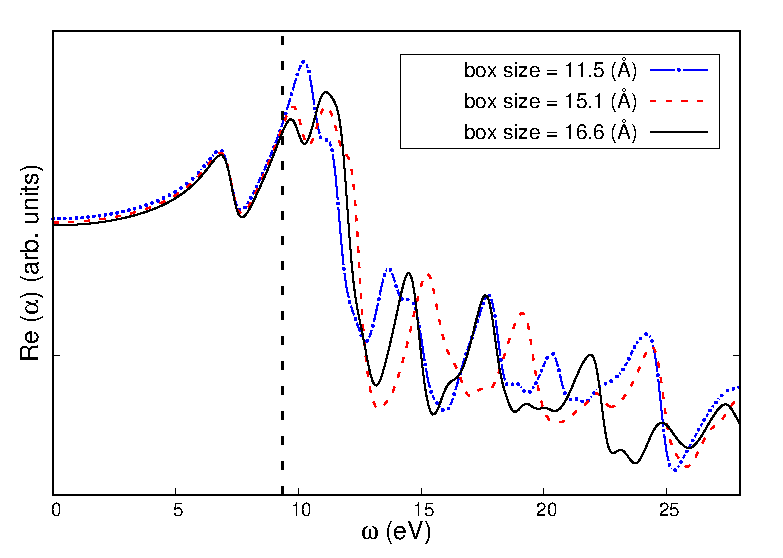
\includegraphics[scale=0.56]{Fig2a_CO_AlphaOmegaReal.eps}} \\
\centering
\subfloat
{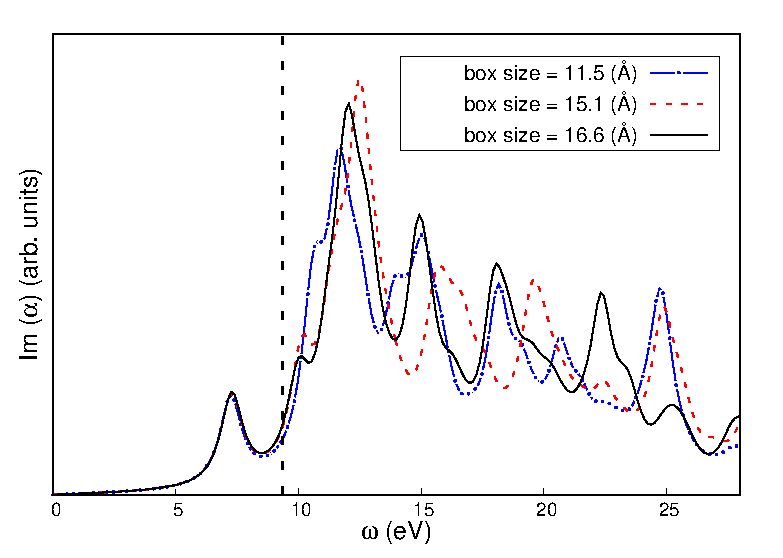
\includegraphics[scale=0.58]{Fig2b_CO_spectrum.eps}}
\caption{\label{co_spectrum}(Color online) LR dynamical polarizability of the $CO$ molecule in computational setups with different
sizes of the simulation domain. The top panel displays the real part and the bottom one the imaginary part. The value of the IP threshold
is indicated by a vertical dashed line.}
\end{figure}

\section{Excitation operators. The analytic structure of the susceptibility functional}

It is possible to reformulate this type of analysis by directly looking at LR quantities that are defined independently from the perturbing operators and target observable. This can be achieved by studying the \emph{susceptibility functional}, defined implicitly trough the operator equation
\be\lb{ExcitationOperatorsDef1}
\Liouv \op E_a = \Omega_a \op E_a \qq \op{\tilde E}_a \Liouv = \Omega_a \op{\tilde E}_a \;,
\ee
together with the operator orthonormalization condition %$\trace{\op{\tilde E}\op E'} = \delta(E-E')$.
\be\lb{orthoExcitatioOpDef1}
\trace{\op{\tilde E}_a\op E_b} = \delta_{ab} \;.
\ee
Excitations defined in that way may be considered as a basis of the operators that satisfy the transverse condition as in
Eq.~\eqref{RhopTransverseDef1}, and enable us to express the susceptibility as a spectral decomposition:
\be\lb{RhopExcitationDef1}
\sop{{\cal \chi}}(\omega) \cdot   = \sum_{\{a\}} \op E_{a} \,
\frac{\trace{\commutator{\op{\tilde E}_a}{\dmnot}\cdot}}{\omega-\Omega_a} \;.
\ee
In this way Eq.~\eqref{LinearResponseFunctDef2} may be also written as:
\be\lb{deltaoexc}
  \braket{\delta \op O} =  \sum_{\{a\}} \frac{\trace{\op O \sop B_a \op \Phi(\omega)}}{\omega -\Omega_a}\;,
\ee
where the action of the spectral operator $\sop B_a$ reads
\be
  \trace{\op O \sop B_a \op \Phi(\omega)} = \trace{\op O \op E_a}
  \trace{\op{\tilde E}_a \commutator{\dmnot}{\op \Phi(\omega)}} \;. \nn
\ee

\subsection{Localization features of the excitation operators. The analytic structure of linear susceptibility}

The properties of the Liouvillian superoperator $\Liouv$ (sketched in appendix \ref{LiouvillianAction}) imply that both the left and right operator-valued
eigenstates \eqref{ExcitationOperatorsDef1} satisfy the transverse condition \eqref{RhopTransverseDef1} and can be parametrized as
\begin{align}\lb{ExcitationOperatorsDef2}
\op E_a &= \sum_p \left( \ket{\phi^a_p}\bra{\psi_p} + \ket{\psi_p} \bra{\chi^a_p}\right)\;, \nn \\
\op{\tilde E}_a = \commutator{\dmnot}{\op E^t_a} &= \sum_p \left( \ket{\psi_p}\bra{\phi^a_p} - \ket{\chi^a_p} \bra{\psi_p}\right)\;.
\end{align}
Each excitation ``mode'' of the system, with associated energy $\Omega_a$, is thus described by a set of states $\{\phi^a_p,\chi^a_p\}_{p \in a}$, defined in the unoccupied subspace. These objects represent, respectively, the state in which $\ket{\psi_p}$ is excited -- or from whom it decays -- when the system is subject to the \emph{monochromatic} perturbation $\op \Phi_a \equiv \commutator{\dmnot}{\op E_a}$. We denote with the shorthand $p \in a$ the fact that the sum of Eq.~\eqref{ExcitationOperatorsDef2} is in general restricted only to a $a$-dependent subset of the occupied orbitals, depending on the particular symmetry
of the excitation. Excited states  satisfy the normalization condition
\be\lb{ExcitedStateOrthNormDef1}
\sum_p \left(\brket{\phi_p^a}{\phi_p^b} - \brket{\chi_p^b}{\chi_p^a}\right) = \delta_{ab} \;.
\ee
By applying \eqref{ExcitationOperatorsDef1} to the above parametrization
of the excitations, we obtain the following Sternheimer-like equations for the excited states:
\begin{align}\lb{ExcitationOperatorsDef3}
&\left[\Omega_a-(\hnot - \eps_p)\right] \ket{\phi_p^a} = \op Q_0 \op V'[\op E_a] \ket{\psi_p} \;, \nn\\
&\bra{\chi_p^a}\left[-\Omega_a-(\hnot - \eps_p)\right] = \bra{\psi_p} \op V'[\op E_a] \op Q_0  \;.
\end{align}
By writing these equations in a basis set of virtual states we obtain the well-known Casida's eigenvalue equation\cite{CasidaBook}
associated to the excitation energy $\Omega_a$ (see appendix \ref{casida}).
The spectrum is symmetric w.r.t the inversion of the eigenvalues $\Omega_a \rightarrow -\Omega_a$ and, given a specific excitation $\{\phi^a_p,\chi^a_p\}$, 
the associated solution with opposite energy is described by the transposed pair $\{\chi^a_p,\phi^a_p\}$.
We concentrate our analysis on the sector of positive energies, i.e. $\Omega_a > 0$.

With the same spirit of the previous sections, we present a formal solution of \eqref{ExcitationOperatorsDef3} as follows
\begin{align}
\ket{\phi^a_p} &= \GH(\Omega_a+\eps_p)\left(\op V \ket{\phi^a_p} + \ket{s_p[\op E_a]} \right) \;, \nn \\
\bra {\chi^a_p} &=\left(\bra{\chi^a_p} \op V  + \bra{s_p[\op E_a]}\right)  \GH(-\Omega_a+\eps_p)\;,
\end{align}
where the source terms are here defined as:
\be
 \ket{s_p[\op O]} =  \op Q_0 \op V'[\op O] \ket{\psi_p}\,, \quad
 \bra{s_p[\op O]} =   \bra{\psi_p} \op V'[\op O] \op Q_0 \nn \;.
\ee
First, we point out that the Helmholtz kernel associated to the $\ket{\chi^a_p}$ state
contains an exponential damping factor for \emph{all} the positive values of $\Omega_a$.
The asymptotic long-range behavior of $\ket{\chi^a_p}$ thus depends only on the locality properties of
$\bra{s_p[\op E_a]}$, which in turn is related to the behavior of the operator $\op V'[\op E_a]$.

On the other hand, the long-range behavior of $\GH(\Omega_a+\eps_p)$ depends from
$\Omega_a$, with a threshold of value $\Omega_a=|\eps_p|$.
For energies above this value, the behavior of the state $\ket{\phi^a_p}$ is
delocalized regardless of the particular nature of the operators $\op V$ and $\op V'$.
This means that, if an excitation operator $\op E_a$ has an energy such that
$\Omega_a>|\eps_p|$  for at least one of the $p \in a$ defining the excitation,
such operator \emph{cannot} be parametrized by employing localized states only.

As a consequence, we deduce that a molecular excitation \emph{may} be expressed in terms of localized states
\emph{only} when its energy is lower than \emph{all} the ionization potentials of the occupied states participating to the excitation,
namely if $\Omega_a<|\eps_p|$ $\forall p \in a$. This will only be true if the operator
$\op V'[\op E_a]$ can be restricted to localized kets and bras.
If any of these hypothesis does not hold, the excitations of the systems are defined via genuinely delocalized wavefunctions.
Furthermore, excited states are subjected to the orthonormalization condition
\eqref{ExcitedStateOrthNormDef1} that acts as a ulterior constraint and has the effect of determining the \emph{quantization}
of the energy levels $\Omega_a$ associated to the bound-state-like objects.
For delocalized states, as in the case of the continuum states of $\hnot$,
such a condition has to be interpreted in distributional sense and does not lead to quantization of $\Omega_a$.
Thus we can conclude that all the states $\ket{\chi^a_p}$ and the $\ket{\phi^a_p}$ with $\Omega_a$ below the threshold value constitute
-- if localized -- a genuine \emph{discrete} set, while the ones in the unbound energy range behaves as generalized eigenvectors associated to a
continuum spectrum.

%%%%%%%%%%%%%%%%%%%%%%%%%%%%%%%%%%%%%%%%%%%%%%%%%%%%%%%
\begin{figure}[!t]
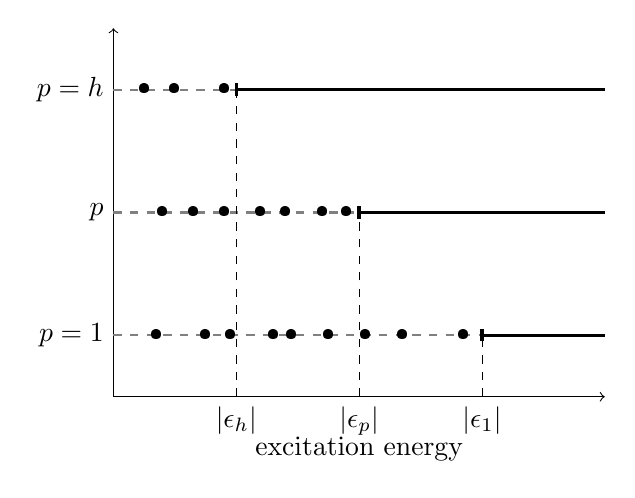
\begin{tikzpicture}[scale=0.78]
% axes
\draw[->] (0,0) -- (8,0);
\draw[->] (0,0) -- (0,6);
% orizontal lines
\draw[dashed,thick,color=gray] (0,5) -- (2,5);
\draw[very thick](2,5) -- (8,5);
\draw[dashed,thick,color=gray] (0,3) -- (4,3);
\draw[very thick] (4,3) -- (8,3);
\draw[dashed,thick,color=gray] (0,1) -- (6,1);
\draw[very thick] (6,1) -- (8,1);
% % vertical lines
\draw[dashed,very thin,color=black] (2,0) -- (2,5);
\draw[dashed,very thin,color=black] (4,0) -- (4,3);
\draw[dashed,very thin,color=black] (6,0) -- (6,1);
% % threshold levels labels
\node[left] at (0,5) {$p=h$};
\node[left] at (0,3) {$p$};
\node[left] at (0,1) {$p=1$};
\node[below] at (2,0) {$|\eps_h|$};
\node[below] at (4,0) {$|\eps_p|$};
\node[below] at (6,0) {$|\eps_1|$};
\node[below] at (4,-0.5) {excitation energy};
% bars at thresholds
%\foreach \Point in {(2,5),(4,3),(6,1)}{
%   \node at \Point {{\textbar}};%$\times$};
%}
\draw[very thick] (2,4.9) -- (2,5.1);
\draw[very thick] (4,2.9) -- (4,3.1);
\draw[very thick] (6,0.9) -- (6,1.1);
% dotted vertical lines
%\draw[dotted,thick,color=black] (-0.2,3.6) -- (-0.2,4.4);
%\draw[dotted,thick,color=black] (-0.2,1.6) -- (-0.2,2.4);
% discrete excitations
\foreach \Point in {(0.5,5),(1.0,5),(1.8,5),(0.8,3),(1.3,3),(1.8,3),(2.4,3),(2.8,3),(3.4,3),(3.8,3),(0.7,1),(1.5,1),(1.9,1),(2.6,1),(2.9,1),(3.5,1),(4.1,1),(4.7,1),(5.7,1)}{
    \node at \Point {\textbullet};
}
\end{tikzpicture}
\caption{\label{ExcitationLandscape} Excitation landscape. Excitations are split in horizontal line according to the threshold levels $p$. Filled bullets refer to localized
excitations whereas the thick black lines describe delocalized ones belonging a continuum spectrum.}
\end{figure}
%%%%%%%%%%%%%%%%%%%%%%%%%%%%%%%%%%%%%%%%%%%%%%%%%%%%%%%

The susceptibility functional has therefore a peculiar analytic structure made of multiple threshold energies, one for each of the ionization potentials associated to the occupied states. If an excitation $\op E_a$ has an energy $\Omega_a < |\eps_a|$ with $\eps_a = \mathrm{max}\left(\eps_p\right)_{p\in a}$, it may belong to a discrete spectrum; otherwise it \emph{has} to belong to a continuum of states.
The typical structure of the excitation landscape is depicted in figure \ref{ExcitationLandscape}, once again assuming that the perturbed potential $\op V'[\op E]$ gives rise to a bound state when applied to $\ket{\psi_p}$. Below the first ionization energy $|\eps_h|$ only localized excitations are present. Conversely, in the intermediate energy interval that extends from $|\eps_h|$ to the absolute value of the deepest occupied orbital, other discrete excitations may exist, and are embedded in a continuum of delocalized excitations. For energies higher than $|\eps_1|$ \emph{no localized} excitations are anymore possible,
regardless of the particular behavior of $\op V'$: the excitation landscape in this region contains a continuum set of delocalized states.

\section{Physical relevance of the excitation spectrum. A comparison among localized and continuum sectors}
% \deleted[id=dal]{
% Comments on the features and the physical relevance of the two sector of the excitation spectrum}
% 
% %\subsection{Localized sector}
% 
% %\begin{itemize}
% % \deleted[id=dal]{\item It is composed by a genuine set of discrete elements.}
% % \deleted[id=dal]{\item The values of the excitation energies do not depend on the computational setup (observable features) and so can be compared among different approaches.}
% % \deleted[id=dal]{\item The knowledge of this sector of the excitation spectrum allows us to express only the imaginary part of (proper equation that expresses the response functional written using Sokowsky-Plemely
% % on the susceptibility functional).}
% % \deleted[id=dal]{\item A computational setup in which delocalized degrees of freedom are excluded by design can in principle describe to this sector in a exact way.}
% %\end{itemize}
% 
% \subsection{Continuum sector}
% 
% \begin{itemize}
%    \item Make some statements on the features that a computational setup must have to guarantees that this sector provides converged results. Difference between systematic and localized basis setup. Can we comment about the needs to add ghost atoms for the evaluation of statical polarizability with gaussian basis?
%  % \deleted[id=dal]{\item Not true poles of the susceptibility (but only an effective tool to compute the spectral function).}
%  % \deleted[id=dal]{\item Deeply affected by the computational setup used to represent them. In particular, the presence of a finite computational domain implies a fictitious discretization of the excitation levels and the associated spectrum exhibits an explicit dependence from the size of the domain.}
%  % \deleted[id=dal]{\item This sector of the excitation spectrum is needed to compute imaginary parts above IP and real part for \emph{all} the values of $\omega$. Add examples on the statical polarizability. Can we comment}
% \end{itemize}
% 
% 
% \vspace{1cm}

\subsection{Observable features of the excitation spectrum}

The analysis of the above section reveals that the excitation spectrum is composed by two distinct sectors.
The first one is realized by the (finite) set of localized excitations with discrete eigenvalues.
Borrowing the terminology introduced in section \ref{SEopenSystem} to the present case, we can affirm that such localized excitations behave as
\emph{observable} quantities and the associated energies possess ideal features of reproducibility:
if the numerical basis employed is complete enough to
represent the states $\{\phi_p^a,\chi_p^a\}$, the energy $\Omega_a$
converges to its reference value.
A computational setup in which delocalized degrees of freedom are excluded by design can, in principle, describe excitations of this sector in a exact way.

The second sector contains a continuum spectrum of delocalized excitations. The associated states $\ket{\phi_p^a}$ behave as the unbound virtual orbitals analyzed in \cite{boffi2016}
and are deeply affected by the computational setup used to represent them. In particular, the presence of a finite computational domain implies a fictitious discretization of the excitation levels and
the associated spectrum exhibits an explicit dependence from the size of the domain.
Excitations belonging to this sector thus lose their intrinsic physical meaning and have to be understood simply as objects providing an effective representation of the density of states (DOS) of the Liouvillian superoperator.

\begin{figure}[ht]
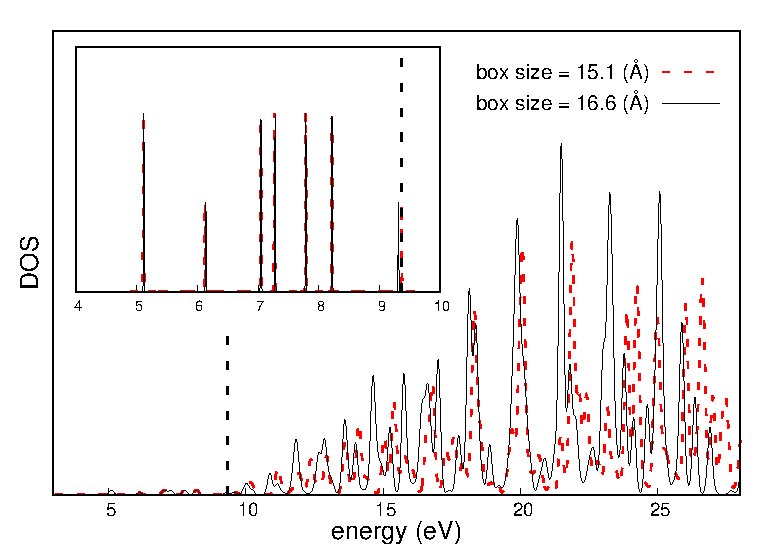
\includegraphics[scale=0.6]{Fig4_CO_dos_rev1.eps} %{Fig4_CO_dos.eps}
\caption{(Color online) DOS of $CO$ excitation energies $\Omega_a$. The two curves correspond to two computational domain of different sizes. The inset contains the sole contribution of localized excitations. The first IP threshold is depicted as the vertical dashed line.}
\label{CO_exc}
\end{figure}
\begin{figure}[ht]
\centering
\subfloat[Excitation landscape]
{\label{c6h6_excLand}
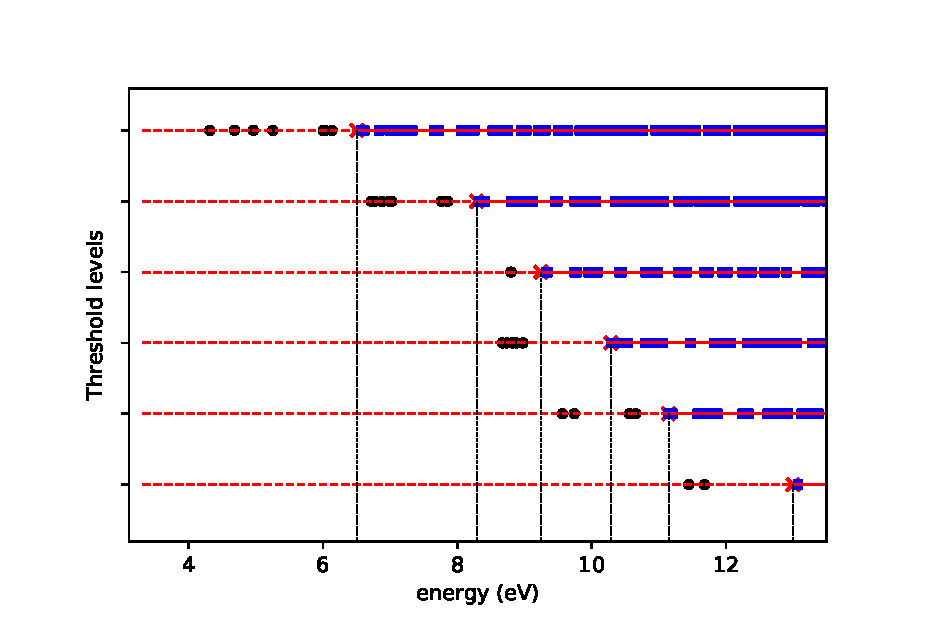
\includegraphics[scale=0.56]{Fig5a_C6H6_excLandscape.eps}} \\
\centering
\subfloat[DOS of Excitation energies]
{\label{C6H6_exc}
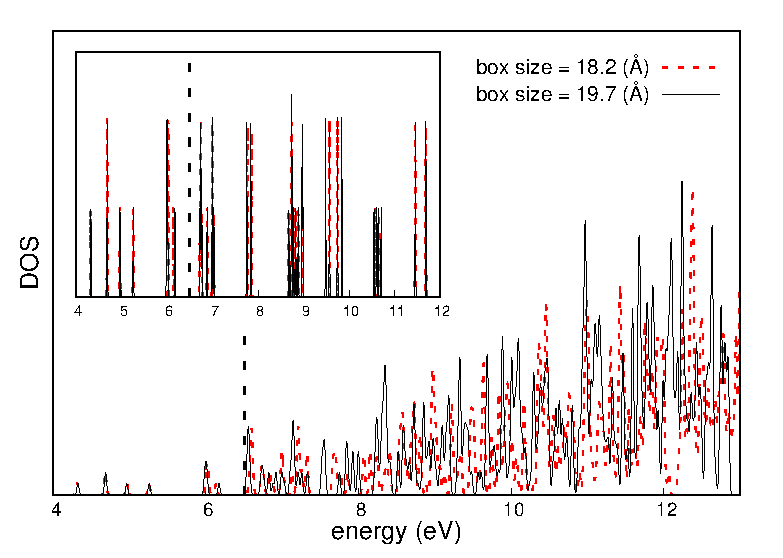
\includegraphics[scale=0.58]{Fig5b_C6H6_dos_rev1.eps}} %{Fig5b_C6H6_dos.eps}
\caption{(Color online) Benzene molecule. (a): Excitation Landscape: the excitations have been separated in discrete and continuum sector following the criteria of Sec.~\ref{ExcitationLandscape}. (b): DOS of excitation energies $\Omega_a$. The first IP threshold is depicted as the vertical dashed line.}
\end{figure}

In Fig.~\ref{CO_exc} and \ref{C6H6_exc} we plot the DOS of the Liouvillian for the $CO$  and Benzene molecules,
for two different numerical setups of increasing size of the simulation domain.
The figures show clearly that all the excitations of energy $\Omega_a$ lying below the
molecule ionization potential (IP) have a localized behavior, as their energy does not vary with the size of the simulation domain.
On the other hand, above the first ionization threshold the excitations have an energy that strongly depends on the computational
setup, which is in line with the expected pseudo-continuum character of this sector.
In addition, for the benzene molecule it is also possible to
identify excitations of energy above IP that still possess a localized behavior, fulfilling the condition $\Omega_a < |\eps_a|$.
In Fig.~\ref{c6h6_excLand} we collect the excitations of the benzene molecule following this criterion:
the agreement with the expected analytic structure presented in Fig.~\ref{ExcitationLandscape} is remarkable.

\subsection{Relative importance of discrete and continuum excitations}
% \deleted[id=gen]{
% We have presented formal arguments, confirmed by numerical calculations, that show that
% the excitations belonging to the discrete sector of the spectrum have energies
% that can be \emph{quantitatively} compared between codes, thanks to their
% localized character.
% Such objects are LR quantities, associated to the molecule, whose numerical convergence
% can be found by employing techniques which can be borrowed from the ones adopted for GS calculations. Being expressed by localized excited states,
% computational setups with sufficient level of completeness are able to
% express with high \emph{precision} such section of the excitation spectrum.}

So far we have showed with both formal arguments and numerical calculations that the excitation spectrum split into two sectors with very different features.
It is so reasonable to ask which is the relative importance of these two sectors and in particular if there is the possibility to express observable quantities
in a suitable $\omega$ range, by only employing the sector of genuinely localized excitations.
% We may ask which is the relative importance of the two sectors and in particular if there is the possibility to express observable quantities
% in a suitable $\omega$ range, by only employing the sector of genuinely localized excitations.
Stated otherwise, will the \emph{restriction} of $\sop \chi(\omega)$ to only localized excitations can be useful to extract some physical quantities?

In this regard it is illustrative to apply the above arguments to the evaluation of the dynamical polarizability tensor $\alpha_{ij}(\omega)$.
Employing the formalism of Eq.~\eqref{deltaoexc} provides
\be%gin{align}
  \mathrm{Im}\left(\alpha_{ij}(\omega) \right) =
  \sum_{a} \trace{\mathbf r_i \sop B_a \mathbf r_j} \delta(\omega - \Omega_a)\lb{imalpha} \;.
  %\\
  % &= 2 \sum_p \bra{\psi_p} \mathbf r_i \left(\mathrm{Im}\ket{f_p^{\mathbf r_j}(\omega)}\right)\lb{imfs}\;,
\ee%nd{align}
The imaginary part of the dynamical polarizability tensor therefore can be seen as the partial density of states of the Liouvillian projected on
$\op{\mathbf r}_i\op{\mathbf r}_j$. For this reason, it is evident that below the \emph{first} excitation threshold (IP), the contributions to $\mathrm{Im}\left(\alpha_{ij}(\omega)\right)$ can be expressed only in terms of observable excited states. On the contrary, the non-observable, basis dependent continuum sector of the excitation starts to contribute to $\mathrm{Im}\left(\alpha_{ij}(\omega)\right)$ above IP; the localized sector is not anymore sufficient to express Eq.~\eqref{imalpha} in this $\omega$ range.

% Not surprisingly this behaviour is in coherency with the
% localization properties of the FS below IP; Eq.~\eqref{imfs} show that
% for its imaginary part.

%
% The imaginary part of the FS may be decomposed in two quantities:
%
%
% \deleted[id=gen]{
% Following the considerations of Sec.~\ref{FluctuationState}, we know that
% for $\omega$ below the IP threshold all these quantities may be expressed
% via asymptotically localized states.
% We have also seen in Sec.~\ref{FluctuationState} that
% there exist a sector where the fluctuation states are genuinely localized, thereby presenting reproducibility features. Therefore,
% knowing that $\ket{f_p^\Phi(\omega)} =\sop \chi(\omega) \op \Phi(\omega) \ket{\psi_p}$,
% it would be interesting to obtain information on whether the discrete, localized sector of the excitations which appear in the spectral decomposition of $\sop \chi(\omega)$
% will be sufficient to express a localized FS.
% Considering Eq.~\eqref{SusceptibilityDef1} and
% expressing the spectral decomposition of the linear susceptibility we find:}
% \be
% \mathrm{Im}\left(\ket{f_p^{\mathbf r_j}(\omega)} \right)= \fscd{D} + \fscd{C}
% \lb{FSExcitationDef1} \;,
% \ee
% with
% \begin{align}
%  \fscd{D} &= \sum_a^{|\Omega_a| < |\eps_a|} \ket{w_p^a} \bra{\psi_p} \op {\mathbf r}_j \ket{w_p^a} \delta\left(\omega-\Omega_a\right) \;, \nn \\
%  \fscd{C}
%  &= \int_{|\Omega_a| > |\eps_a|} \!\!\!\!\!\!\!\!\!\!\!\!\!\dd a \ket{w_p^a}  \ket{w_p^a} \bra{\psi_p} \op {\mathbf r}_j \ket{w_p^a} \delta\left(\omega-\Omega_a\right) \;, \nn
% \end{align}
% where %$\varphi_p^a[\op \Phi(\omega)] \equiv \bra{\psi_p}\op\Phi(\omega)\ket{w_p^a}$, and
% $\ket{w_p^a}=\ket{\phi_p^a}+\ket{\chi_p^a}$.
%
% In the above equation we have explicitly separated the contributions of the discrete ($D$) and continuous ($C$) excitations
% in the spectral decomposition \eqref{SusceptibilityDef1}.
% \deleted[id=gen]{The summation and the integration run only on the positive values of $\Omega_a$.}
% The states $\ket{w_p^a}$ that appear in the discrete sum
% or in the integral are genuinely localized and delocalized, respectively.
% For \emph{any} value of $\omega$ the ket $\fscd{D}$ has, by definition, a bound-state like
% character as it is expressed as a sum of localized contributions.
%
% It is easy to see that for $\omega$ below IP  we have $\fscd{C}=0$.
% Below threshold, continuum excitations \emph{do not} contribute to the imaginary part of the
% dynamical polarizability.

Let us now consider the features of the response density operator of Eq.~\eqref{rhoPrimeFluctuationStateDef1}.
The fluctuation state in this case can be written as
\be\lb{fsinexc}
\ket{f_p^{\mathbf r_j}(\omega)}=
\sop \chi(\omega) \op{\mathbf r_j} \ket{\psi_p}
= \sum_a \frac{\bra{w_p^a} \op{\mathbf r_j} \ket{\psi_p}}{\omega^2 - \Omega_a^2}
\ket{w_p^a}\;.
\ee
Here we have employed the notation $\ket{w_p^a}=\ket{\phi_p^a}+\ket{\chi_p^a}$.
The above equation shows that for \emph{any} value of $\omega$ both sectors of localized and delocalized states $\ket{w_p^a}$ contribute.
However the discussion of Sec.~\ref{FluctuationState} has shown that
the FS is a genuinely localized state below the IP threshold.
The equivalence of the Sternheimer formalism with the spectral representation of the LR susceptibility implies that in this regime the contribution of the delocalized excitations in Eq.~\eqref{fsinexc} has to resum into a localized, asymptotically vanishing FS.
Such a locality is evident for the imaginary part of the FS, which
can be straightforwardly restricted to the sum over $\ket{w_p^a}$ below IP (see Eq.~\eqref{imalpha}). For the real part of FS the \emph{entire} spectrum
of excitations contribute.

Hence, contrary to GS, \emph{for LR calculation,
even when the response density is localized, the contribution coming from the
continuum sector of the excitations can never be neglected}.
In other terms, we \emph{cannot} exclude that a fluctuation state, even if genuinely localized, will have a nonzero projection
in the essential part of the Liouvillian spectrum.
This fact shows that it is \emph{impossible} to restrict the spectral representation
of $\chi(\omega)$ to only localized, discrete, \emph{code-independent} excitations, even for representing LR results in the $\omega=0$ limit.



% For $\mathrm{Re}\ket{f_p^{\mathbf r_j}(\omega)}$ the situation is slightly more complicated.
% \begin{align}
%   \mathrm{Re}\left(\alpha_{ij}(\omega) \right) &= \mathcal P \int \dd \omega'
%   \frac{\mathrm{Im}\left(\alpha_{ij}(\omega')\right)}{\omega - \omega'} \\
%   & =   \sum_{a} \mathcal P  \frac{\trace{\mathbf r_i \sop B_a \mathbf r_j}}{\omega - \Omega_a}\\
%   & =2 \sum_p \bra{\psi_p} \op O \left(\mathrm{Re}\ket{f_p^{\mathbf r_j}(\omega)}\right)\;.
% \end{align}
% Such equations are in coherency with the Kramers-Kronig relations of the fluctuation states, see Eq.~\eqref{KKrel}.
%
%
% For $\omega <$ IP, we know that the FS is localized.
%
%
% The equivalence of the Sternheimer formalism with the spectral representation of the LR susceptibility implies that the integral of the Kramers-Kronig
% relation ~\eqref{KKrel} involving the delocalized states
% $\fscd{C}$ should resum into a localized, asymptotically vanishing state\footnote{There is no particular reason to believe that $\fscd{C}$ should be
% zero. Since $\ket{w_p^a}$ states are linearly independent,
% $\fscd{C}=0$ would imply
% $\bra{\psi_p} \op {\mathbf r}_j \ket{w_p^a}$ for any $a$ labelling the continuum excitations, which is too strong a condition.}.

% We may then decompose the linear response functional of Eq.~\eqref{LinearResponseFunctDef1}
% for any operator $\op O$ as $\braket{\delta\op O}_\Phi=\braket{\delta\op O}^D_\Phi +
% \braket{\delta\op O}^C_\Phi$, where
% \be
% \braket{\delta\op O}^{D,C}_\Phi(\omega) =
% 2 \bra{\psi_p} \op O \fscd{D,C}\;.
% \ee

\subsection{Effective representation of $\sop \chi(\omega)$ for localized response densities}
The above arguments have shown that the only quantity which can be expressed in terms
of the localized sector of the excitation spectrum is the imaginary part of the
susceptibility functional $\sop \chi(\omega)$ in the optical regime (i.e. $\omega <$  IP).
The response densitites for a generic perturbation and $\omega$ value always require the
inclusion in the Liouvillian DOS of the delocalized part of the excitation spectrum, even in view of expressing localized fluctuation states.

It appears therefore important to identify indicators that might assess the capability of
$\sop \chi(\omega)$ to express localised FS (and thus the complete response density $\dm'_\Phi(\omega)$) below the IP threshold.
For instance, the static polarizability tensor $\alpha_{ij}$ can be calculated as
\be\lb{sminus2}
\alpha_{ij} = \sint \dd a \frac{w^a_{ij}}{\Omega_a^2}\,, \quad w^a_{ij} \equiv \sum_{p\in a} \bra{\psi_p} \op {\mathbf r}_i \ket{w_p^a}\bra{\psi_p} \op {\mathbf r}_j \ket{w_p^a}\;.
\ee
% The summation above runs on both localized and delocalized sector of the excitations.
%
% We also know that $\alpha_{ij}$ might be expressed with arbitrary precision by only employing localized quantities.
Such value can be straightforwardly compared with results of Eq.~\eqref{staticalpha}, where the localized FS is obtained from GS techniques as
described in Sec.~\ref{FluctuationState}.
This is the well-know $S_{-2}$ sum-rule (see e.g.\cite{Wagner2012}), that express the value of the static polarizability
in terms of the molecule's oscillator strengths.
In the context of a numerical evaluation of the excitations, such sum rule can therefore interpreted as the capability of the pseudo-continuum sector of the excitation to
express the localized FS -- and consequently the reference value of $\alpha_{ij}$ -- at $\omega=0$.

We have analized the fullfillment of Eq.~\eqref{sminus2} for moeculs of various
sizes and symmetries.
In Fig.~\ref{co_AlphaExc} we show explicitly such a comparison in the case of the $CO$ molecule.
We notice that a considerable number of pseudo-continuum excitations is required
to find the correct result; the sector of the discrete excitations, even though
parametrised by localized, observable (in the sense of reproducible) excited states,
appears to be largely insufficient to express the reference fluctuation state. Its contribution is even negligible w.r.t.
the one coming from the continuum sector.

\begin{figure}
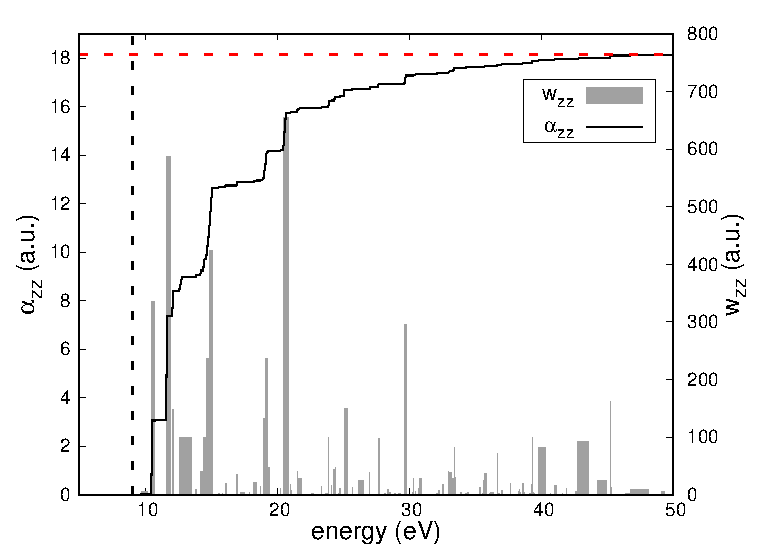
\includegraphics[scale=0.6]{Fig6_CO_statPolvsExc.eps}
\caption{\label{co_AlphaExc}(Color online) Convergence of the statical polarizability $\alpha_{zz}$ of the $CO$ molecule, in a box of $11.5$ \AA,
w.r.t the excitations considered in the integral of Eq.~\eqref{sminus2}. The reference value obtained from Eq.~\eqref{staticalpha} is represented as a
horizontal red dashed line. The value of the IP energy is indicated by a vertical black dashed line. For each excitation energy, the values of the
oscillator strengths $w^a_{zz}$ of Eq.~\eqref{sminus2} are also plotted. }
\end{figure}

Present the table of the other results.

Such a scenario can be also found in the other molecules we have considered;
varying the molecule size and symmetry seems not to modify the qualitative behaviour of the excitation landscape. In addition the
localized sector of the excitations alone is largely insufficient to express $\alpha_{ij}$.
Such considerations are independent on the number of atoms of the molecule, as the range in $\omega$ needed to
achieve satisfactory agreement is largely above the last valence ionization threshold, which is
a intensive quantity.

Once again, this proves that, for any numerical treatment,  pseudo-continuum excitations are fundamental in view of a correct expression
of the response density below IP.
However, the fulfillement of $S_{-2}$ is not a universal quality indicator of $\chi(\omega)$ as the latter may be still badly represented in the high frequency regime:
it is enough to recall
the strong dependency on the box size of the absorption spectra of Fig.~\ref{CO_exc}.
For all these computational setups, the $S_{-2}$ sum rule is, on the contrary, well satisfied.


\section{Conclusions and Perspectives}
We have performed a critical assessment of the fundamental equations
that govern the Linear Response theory of molecular systems.
We have
%By analysing the fundamental equations of LR calculations of molecules, we have
shown that the response density for values of $\omega$ above the first IP
\emph{has} to be expressed in terms of genuinely delocalized states. This
result
has relevant consequences in the choice of the  approptiate computational
basis set to be employed for the LR treatment.

For frequencies below the IP threshold,
under reasonable assumptions on the perturbing operators,
the response density is genuinely localized.
In this regime, it is possible to achieve convergence of the numerical result
by increasing the basis completeness in the same spirit of GS calculations.
More complete basis sets will provide more precise results, regardless of their asymptotic behavior.
A comparison among various computer codes in view of reproducibility should therefore be performed
initially in this regime.

% The situation is not so simple in the above-threshold regime.
%In this case what is important is the matrix element of the observable of interest
%between the bound, occupied state and the fluctuation state (FS).
%The FS is here an unbound, delocalized function, and a numerical treatment tailored for localized functions will \emph{never} be able to discretise such function with arbitrary accuracy.
% To achieve numerical convergence, care should be taken in expressing accurately the FS on the
% appropriate region of space.
%In view of reproducibility, computational setups which are able to express precisely
%delocalized states seem more interesting in this regime.


From a computational perspective, a set of localized basis functions,
which \emph{by design} excludes long-range oscillatory behaviour,
may be complete enough to express $\sop \chi(\omega)$ \emph{below} IP,
but it will never be able to capture the entire features of the
response density operator above the ionization threshold:
the system's excitations expressed in this basis are reliable \emph{only} in the optical regime. The excitation density of states for $\omega >$ IP
has to be considered as a effective representation of $\sop \chi(\omega)$
in order to fulfill Eq.~\eqref{fsinexc}. This fact has been pointed out several times (see e.g. \cite{giustino2012,giustino2014}) in the literature.
High-energy excitations belong to a continuum sector, which should not be
confused
%that embeds the above mentioned discrete excitations.
%We remark that we are not referring here to
with the continuum eigenstates of the
unperturbed GS Hamiltonian.
% but to the continuum of excitations expressed as eigenstate of the
% Liouvillian superoperator of Eq.~\eqref{LiouZeroDef1}, needed to
% express the spectral representation of the linear susceptibility.

On the contrary, computational treatments that are able to express
delocalized states may be such to describe more efficiently the
excitations DOS, especially because of the capability of the basis to
capture oscillatory behaviour. Like in localized basis sets,
excitations below threshold can be precisely calculated
with the same paradigm of traditional GS calculations.
However, in this computational setup, to correctly express
the linear susceptibility below IP -- more specifically the real part of the fluctuation state -- care should be taken in considering enough delocalised excitations to guarantee fulfillment of sum-rules like Eq.~\eqref{sminus2}.


%
% Such point of view have also enabled us to shed light on the analytic structure of the
% linear susceptibility, which is an intrinsic property of the molecule and does not depend on
%  the perturbing fields.
%  In particular, we have concentrated our interest in its spectral representation in
%  terms of ``free oscillation'' (i.e. excitations) of the system.
%  We have found that \emph{not all} the excitations have to be considered on equal footing.
%  As the excitation spectrum has several energy thresholds, one per quasi-particle IP,
%  there is a sector of \emph{discrete}, \emph{localized} excitations -- whose energies are
% below the corresponding threshold -- which can be compared among different computational treatments.
% Their energies are \emph{true} poles of the linear susceptibility, the excited states being their residues. We can \emph{quantify} the reliability of such discrete energies, as the corresponding excited states may be discretized with arbitrary accuracy on a localized region.

% On the other hand, the excitation energies which lie above these thresholds are only pseudo-poles of $\chi(\omega)$,
% and will \emph{strongly} depend on the computational setup. This is visible for energies higher than
% IP, and it has been pointed out several times (see e.g. \cite{giustino2012,giustino2014}) in the literature.
% These excitations belong to a continuum sector that embeds the above mentioned discrete excitations.
% We remark that we are not referring here to the continuum eigenstates of the
% unperturbed GS Hamiltonian,
% but to the continuum of excitations expressed as eigenstate of the
% Liouvillian superoperator of Eq.~\eqref{LiouZeroDef1}, needed to
% express the spectral representation of the linear susceptibility.

Our results show that \emph{both} the sectors of the excitations energies have to be considered in view of the extraction of computationally reliable quantities, and this even below the first IP.
For generic LR quantities, which are functionals of the linear susceptibility,
the quality of the $\chi(\omega)$ (super)operator will depend
on the frequency $\omega$ of interest: a given spectral representation may provide high-quality results for static $\omega=0$ regimes, while being
unable to provide convergence for high-energy absorption spectra.
%On the contrary,
Absorption spectra below IP are relatively easy to converge, as they are observables which depend only on localized quantities.
However, the fulfillment of sum rules like the $S_{-2}$ is not \textit{per se}
a guarantee of the quality of high energy absorption spectra.
Moreover, if the basis set employed for the evaluation of the target $\alpha_{ij}$ in  Eq.~\eqref{sminus2} is identical to the one employed for the LR treatment the $S_{-2}$
is trivially satisfied in the basis. It is therefore important to have a set of reference values
in the complete basis set limit.

We believe that these considerations, based on simple manipulations on the fundamental LR equations, will help in increase
the reliability of LR calculations in the community, and in building test-sets that would help in
the \emph{calibration} of present and future computer codes, thereby increasing the predictivity of present-day theoretical approaches.
The example of the static polarizability of molecules
presents ideal features as an initial playground. Work is ongoing in this direction.

\begin{acknowledgments}
We thank Thierry Deutsch for useful comments on the manuscript.
\end{acknowledgments}

\appendix
\section{Transverse operators and right action of the Liouvillian superoperator}\lb{LiouvillianAction}
Given a unperturbed Hamiltonian and density operator, which satisfy $\commutator{\hnot}{\dmnot}=0$, we may decompose a generic operator in two contributions, $\op O=\op O_\parallel + \op O_\perp$, defined as:
\begin{align}
\op O_\parallel &\equiv \dmnot \op O \dmnot + \op Q_0 \op O \op Q_0 \nn \;,\\
\op O_\perp &\equiv \dmnot \op O \op Q_0 + \dmnot \op O \op Q_0 =
\commutator{\dmnot}{\commutator{\dmnot}{\op O}} \;,
\end{align}
with $\op Q_0 =\identity - \dmnot$.
The operator $\op O_\parallel$ is constructed to satisfy
$\commutator{\dmnot}{\op O_\parallel} = \commutator{\hnot}{\op O_\parallel} =0$.
Also, it is easy to verify that given two generic $\op O$, $\op O'$, we have
$\trace{\op O'_\parallel \op O_\perp} =0$.

The projection $\op O_\perp$ is therefore the relevant part for the commutator:
\begin{equation}
\commutator{\dmnot}{\op O} = \commutator{\dmnot}{\op O_\perp} =
\dmnot \op O \op Q_0  - \dmnot \op O \op Q_0 \;.
\end{equation}
The Liouvillian superoperator is therefore constructed such as $\Liouv \op O = \Liouv O_\perp$. In addition, the image operator satisfies the transverse condition
$\left( \Liouv \op O \right)_\parallel =0$.

Here $\op V'$, which expresses the perturbation induced by the density dependence on ground state Hamiltonian, can be conveniently expressed by defining the
\emph{scalar coupling kernel}
\be\lb{CouplingKernelDef1}
U\left[\op O; \op O'\right] \equiv  \int \dd \r \dd \r' \trace{\op O \frac{\delta \op V[\dmnot] }{\delta \rho(\r,\r')}
} \trace{\op O' \ket{\r} \bra{\r'}}\;,
\ee
on the basis of which
\be\lb{VpDef1}
\op V'[\op O]=
\int \dd \r \dd \r' U\left[\ketbra{\r}{\r'};\op O\right] \ketbra{\r'}{\r}\;.
\ee
We notice here in passing that in general $\op V'[\op O_\perp] \neq \op V'[\op O]$.
We assume nonetheless that the scalar coupling kernel is symmetric, i.e. $U\left[\op O; \op O'\right] = U\left[\op O'; \op O\right]$, which is a condition generally satisfied in DFT Hamiltonians.

The action from the right of $\Liouv$ can be assessed through the equivalence $\trace{\op O'(\Liouv\op O)} = \trace{(\op O'\Liouv)\op O_\perp}$, which implies that also
$\left(\op O' \Liouv\right)_\parallel =0$. We obtain:
\be
\op O\Liouv = -\commutator{\hnot}{\op O} + \int \dd\r\dd\r'
U\left[\commutator{\dmnot}{\op O};\ketbra{\r'}{\r}\right]\left(\ketbra{\r}{\r'}\right)_\perp \;. \nn
\ee
With this definition it is explicitly apparent that $\op O\Liouv=\op O_\perp \Liouv$,
similarly to the left action. The action of the Liouvillian reads
\begin{align}\lb{LiouvillianRightActionDef1}
\op O\Liouv &= -\commutator{\hnot}{\op O} + \left(V'\left[\commutator{{\dmnot}}{\op O}\right]\right)_\perp = -\commutator{\hnot}{\op O} + \nn \\
&+ \dmnot\op V'\left[\commutator{{\dmnot}}{\op O}\right]\op Q_0 + \op Q_0\op V'\left[\commutator{\dmnot}{\op O}\right]\dmnot \;.
\end{align}
In the last equivalence we have made usage of the transverse property (see equation \eqref{RhopTransverseDef1}) of the coupling superoperator. The above formulae
together with Eq.~\eqref{LiouZeroDef1} are the starting point for the solution of the eigenvalues equations \eqref{ExcitationOperatorsDef1}.

\section{Casida equations}
\label{casida}

We show that Casida equations are equivalent to the equations of motion for the excited states \eqref{ExcitationOperatorsDef3}. To this aim we introduce an explicit basis $\{\ket{s}\}$
in the subspace of empty states so that both $\ket{\phi^a_p}$ and $\bra{\chi^a_p}$ can be represented as
\be
\ket{\phi^a_p} = \sum_s X^a_{p s}\ket{s} \;, \qq
\bra{\chi^a_p} = \sum_s\bra{s}Y^a_{p s} \;. \lb{phiandchi}
\ee
Plugging this expansion into equations \eqref{ExcitationOperatorsDef3} and projecting on a arbitrary element of the basis provides a linear systems of equations for the coefficients
$X^a_{ps}$ and $Y^a_{ps}$, namely
\begin{align}
 \sum_{s'}(H_{0ss'}-\eps_p\delta_{ss'})X^a_{ps'} + \bra{s}\op V'[\op E_a]\ket{\psi_p} &= \Omega_a X^a_{ps} \;, \nn \\
 -\sum_{s'} (H_{0 s' s}-\eps_p\delta_{s s'})Y^a_{ps'} - \bra{\psi_p}\op V'[\op E_a]\ket{s}& = \Omega_a Y^a_{ps} \;. \nn
\end{align}
Using this basis, excitation operators are expressed as a linear combination of transition operators $\excite{p}{s} \equiv \ketbra{s}{\psi_p}$ and $\decay{s}{p} \equiv \ketbra{\psi_p}{s}$,
as follows
\be\lb{ExcitationOpBasisTransition1}
\op E_a = \sum_{ps}\excite{p}{s}X^a_{ps}+\decay{s}{p}Y^a_{ps} \;.
\ee
The contribution of the coupling operator in the equations of motion of excited states can expressed by means of the coupling kernel \eqref{CouplingKernelDef1} as
\begin{align}
& \bra{s}\op V'[\op E_a]\ket{\psi_p} = \sum_{qs'}\left(U[\decay{s}{p};\excite{q}{s'}]X^a_{qs'} + U[\decay{s}{p};\decay{s'}{q}]Y^a_{qs'}\right) \;,\nn \\
& \bra{\psi_p}\op V'[\op E_a]\ket{s} = \sum_{qs'}\left(U[\excite{p}{s};\excite{q}{s'}]X^a_{qs'} + U[\excite{p}{s};\decay{s'}{q}]Y^a_{qs'}\right) \;, \nn
\end{align}
Give that we employ real functions both for $p$ and $s$ is real we also have $\excite{p}{s}(\r,\r') = \decay{s}{p}(\r',\r)$ and the density operator is symmetric in $\r \leftrightarrow \r'$.
These conditions applied together imply that $U[\excite{p}{s};\excite{q}{s'}] = U[\decay{s}{p};\decay{s'}{q}]$, as well as $U[\decay{s}{p};\excite{q}{s'}] = U[\excite{p}{s};\decay{s'}{q}]$,
and so equations \eqref{ExcitationOperatorsDef3} can be recasted in matrix form
\be\lb{ExcitationMatrixEq1}
\sum_{qs'}\mat{F_{ps}^{qs'} &  D_{ps}^{qs'}  \\
- D_{ps}^{qs'} & - F_{ps}^{qs'} }
\mat{X^a_{qs'} \\ Y^a_{qs'}} = \Omega_a \mat{X^a_{ps} \\ Y^a_{ps}}
\ee
where
\begin{align}
& F_{ps}^{qs'} = (H_{0 ss'}-\eps_p\delta_{ss'})\delta_{pq} + U[\decay{s}{p};\excite{q}{s'}] \;,\nn \\
& D_{ps}^{qs'} = U[\decay{s}{p};\decay{s'}{q}] \;.
\end{align}
This is the well-known Casida Equation in the basis of transitions for the excitation of energy $\Omega_a$. The computational reliability of the
eigenvalue $\Omega_a$ depends on the capability of the basis set $\ket{s}$ to fulfill of Eq.~\eqref{phiandchi}. Note that this may be valid only for a subset of the solutions of the eigenproblem \eqref{ExcitationMatrixEq1}.

\section{Computational details} \lb{compdetails}
The illustrative calculations presented in this paper are all KS-DFT calculations at the LDA level of theory. We employed the BigDFT code \cite{BigDFT},
that make usage of Daubechies Wavelets as computational basis set. This orthonormal basis presents optimal features of in view of reproducibility of the results, and it has proven to represent precisely and explicitly system with Free as well as Periodic boundary conditions (BC), without any basis set superposition error nor supercell aliasing, for Free BC.

For Ground State results, the important parameters in the context of convergence of the calculations are the spacing of the wavelet grid and the size of the simulation domain: for bound-state like functions, convergence is achieved by reducing the grid spacing and increasing the simulation box size.
Norm Conserving Pseudopotentials (PSP) of the HGH \cite{NLCCPSP} type are employed to remove the core electrons. Such PSP have proven to be able to provide all-electron accuracy for molecular systems.

Our LR calculation are performed with the Casida formalism \cite{bhaarathi}, where it is also important to include a sufficient number of unoccupied states in the transition operators. As pointed out in the text such states behave as plane waves: the features of wavelets enable us to represent localized and delocalized states on equal footing.
For each size of the simulation domain, the number of unoccupied states used for building the Casida' eigenproblem has been increased up to convergence of the presented results.

\subsection{$CO$}
The molecule is oriented along the $z$ axis and the $z$-dimension of the box is equal to 11.5, 15.1 and 16.6 \AA.
280 unoccupied states have been computed in each setup, which span an energy range of the empty KS orbitals of 30.7, 19.3 and 15.4 eV respectively.
Such energy values should not be confused with the excitations energy ranges reported in Figs.~\ref{co_spectrum} and \ref{CO_exc}.
Once again, such choices of unoccupied states ensures convergence in of excitations spectrum in the presented range.

The DOS reported in figure \ref{CO_exc} are obtained by adding a smearing parameter of $8\times 10^{-2}$ eV whereas in the inset shift is $5\times 10^{-3}$ eV.

\subsection{Benzene}
The molecule is oriented in the $xy$ plain and the $x$-dimension of the box is equal to 15.0, 18.2 and 19.7 \AA.
220 states have been computed in each setup and the corresponding
energy reange for the unoccupied states is 16.9, 11.6 and 9.7 eV.

The DOS reported in figure \ref{C6H6_exc} are obtained by adding a complex shift of $1.3\times 10^{-2}$ eV whereas in the inset shift is $5\times 10^{-3}$ eV.



%%%%%%%%%%%%%%%%%%%%%%%%%%%%%%%%%%%%%%%%%%%%%%%
%\bibliographystyle{apsrev4-1}
\bibliography{Analytic_biblio}
%%%%%%%%%%%%%%%%%%%%%%%%%%%%%%%%%%%%%%%%%%%%%%%

\end{document}
